\section{System Design}

The Lung Cancer Early Diagnosis and Monitoring system is designed using a modern client-server architecture, consisting of three main components: User Interface (Frontend), Backend Services, and Database.

\subsection{User Interface (UI) Design}

The user interface is built to provide an intuitive and efficient experience for doctors and medical staff.
\begin{itemize}
    \item \textbf{Core Technologies:} React and TypeScript. React was chosen for its rich ecosystem and ability to create dynamic user interfaces. TypeScript enhances code reliability and maintainability through static type checking.
    \item \textbf{Styling:} Tailwind CSS is used for quick and consistent styling. It allows building highly customized interfaces without writing much custom CSS.
    \item \textbf{Component Library:} Using a UI component library (e.g., Shadcn/ui or similar) to provide pre-built components like cards, forms, charts, and tables, helping to speed up development and ensure interface consistency.
    \item \textbf{UI Theme:} Applying a color scheme with light blue tones as the main colors. These colors were chosen to create a sense of trust, professionalism, and readability in clinical settings, reducing eye strain during long periods of use.
\end{itemize}

\subsection{User Flows}
This section describes the main interaction flows of users (doctors) with the system.
\begin{itemize}
    \item \textbf{Overview Flow:} Doctors log in and view the main dashboard with a list of patients and alerts.
    \item \textbf{Patient Detail Flow:} Doctors select a patient from the list to view detailed information, symptom history, and the latest AI prediction results.
    \item \textbf{Information Update Flow:} Doctors update new symptoms or monitoring notes for patients.
\end{itemize}
% (Optional: Add user flow diagram images here if available)
% \begin{figure}[h]
%     \centering
%     \includegraphics[width=0.8\textwidth]{Images/user_flow_diagram.png}
%     \caption{Flow diagram for viewing patient details.}
%     \label{fig:user_flow}
% \end{figure}

\subsection{Mockups}
The images below illustrate the user interface design for the main screens of the application.

\begin{figure}[h]
    \centering
    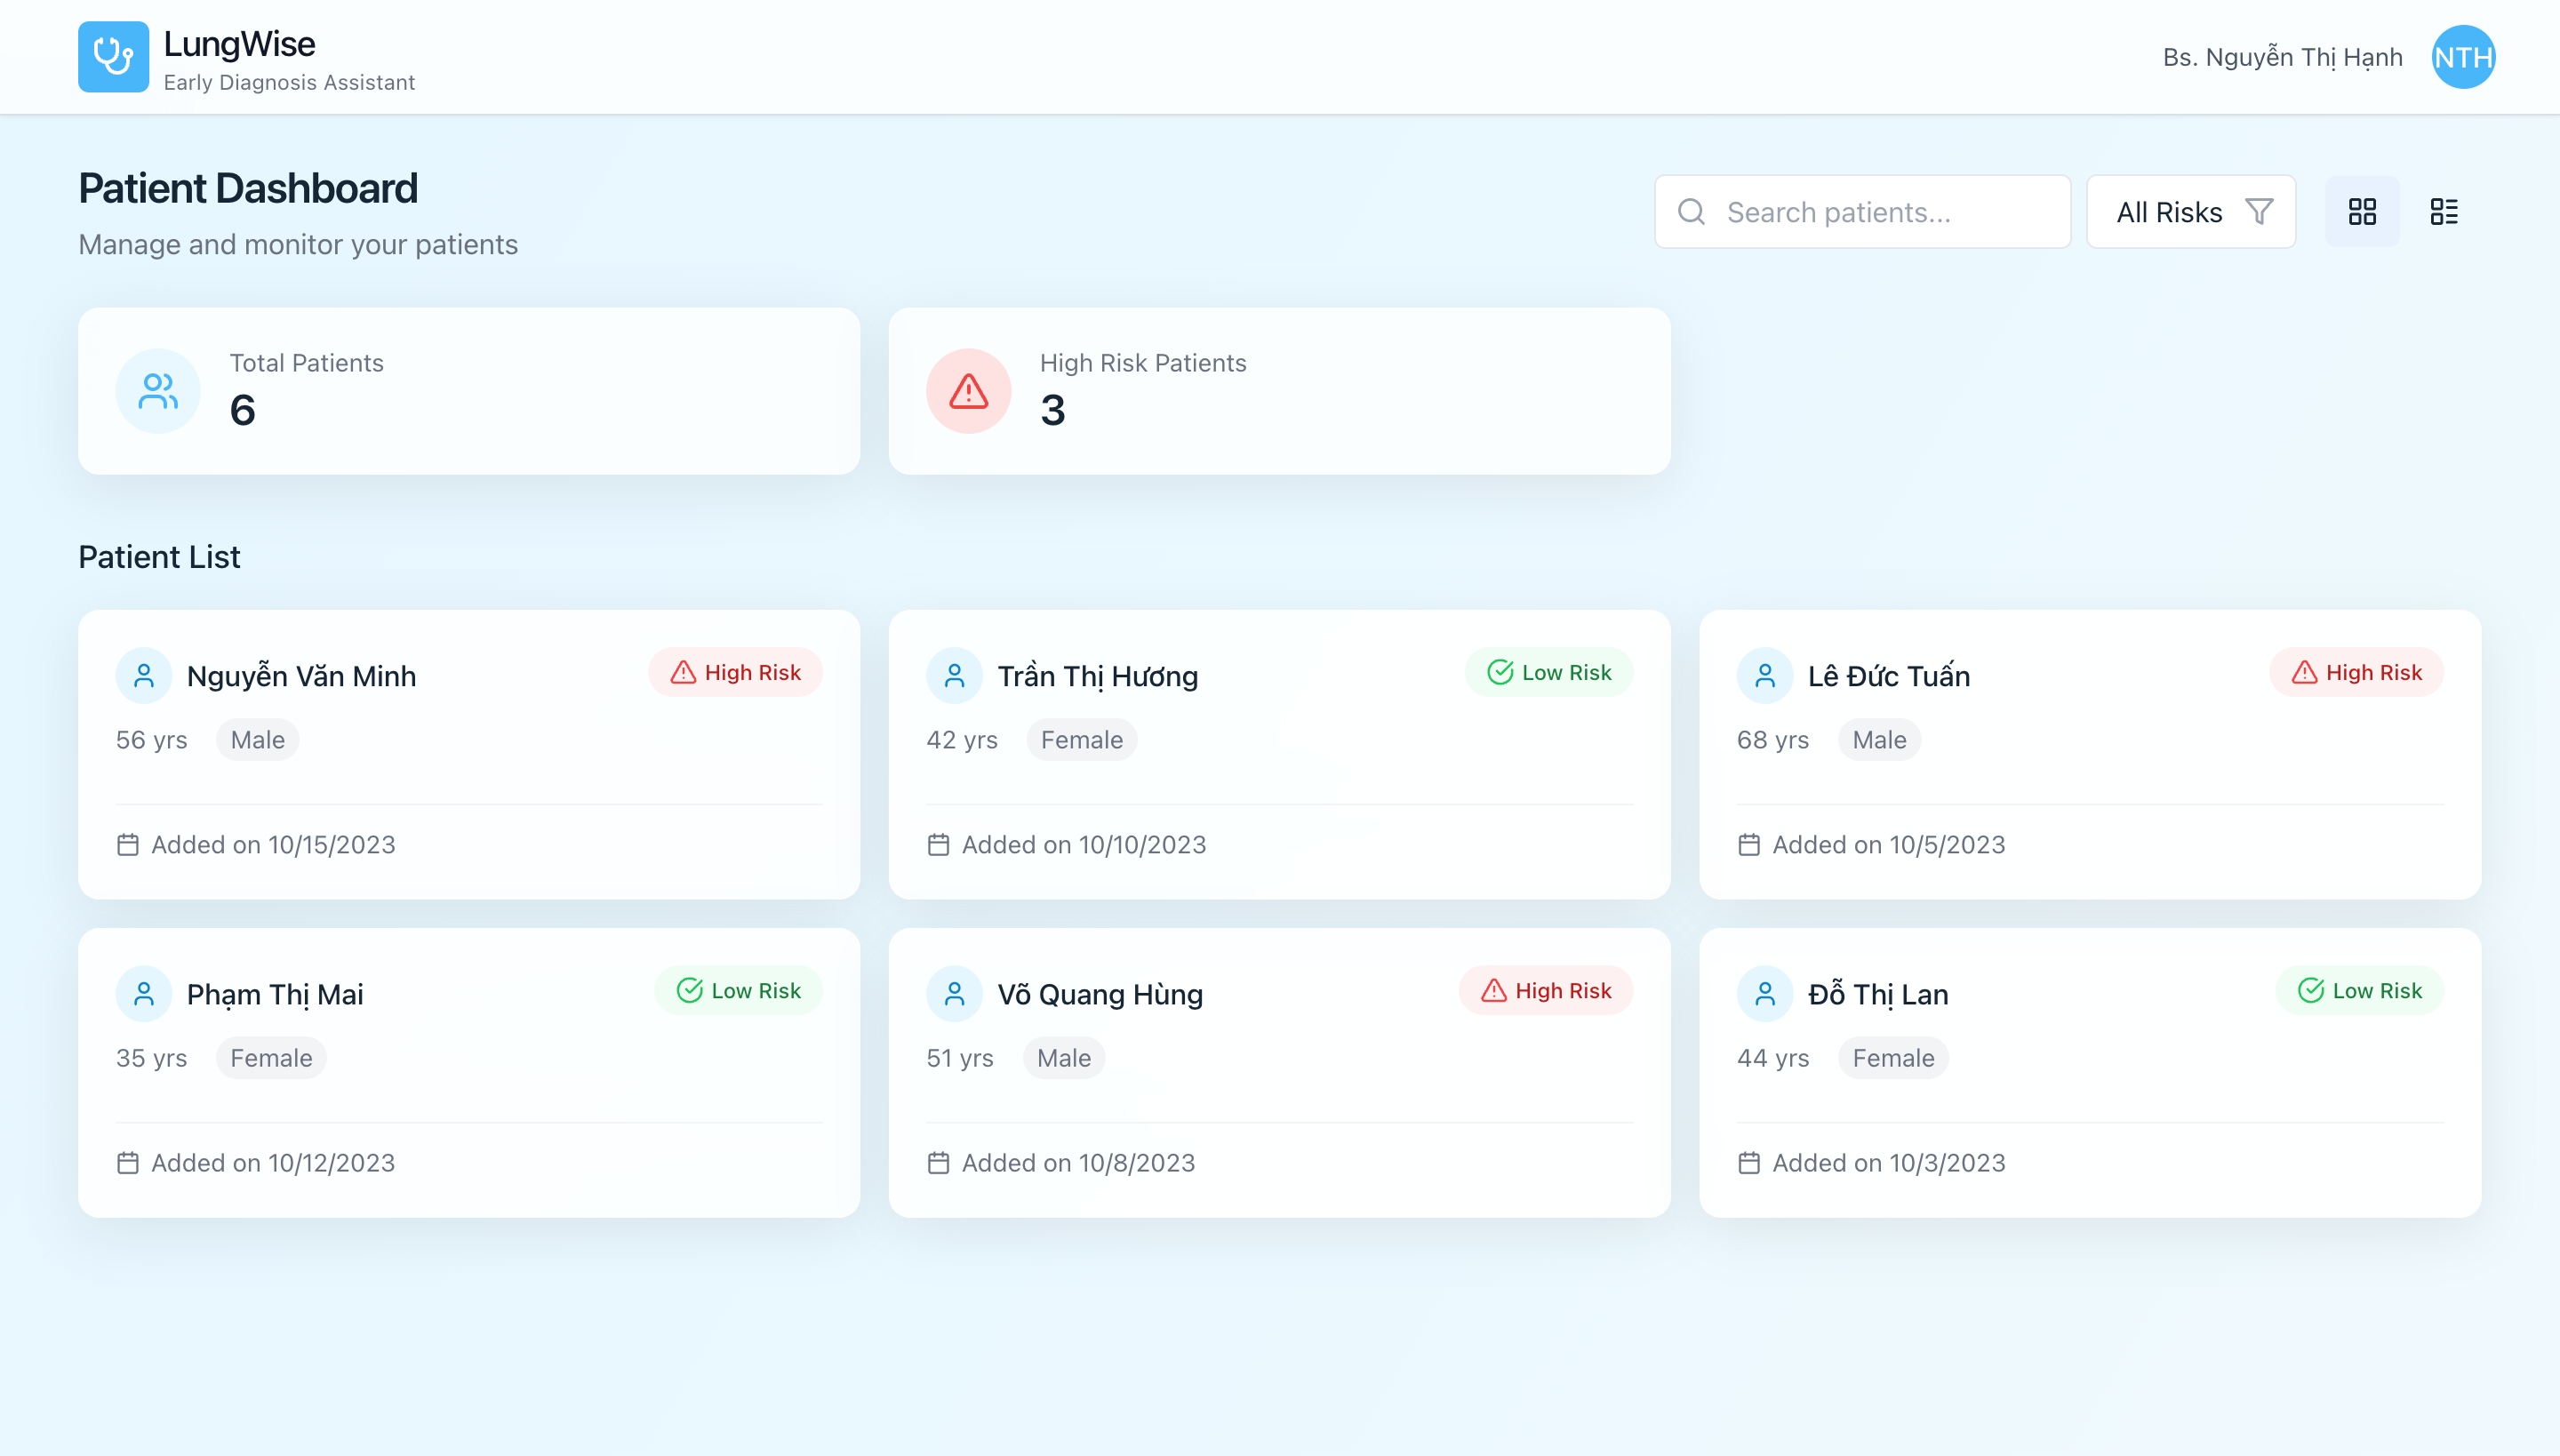
\includegraphics[width=0.9\textwidth]{Images/dashboard.png}
    \caption{The main patient dashboard interface showing patient list, risk categorization, and filtering options.}
    \label{fig:dashboard_mockup}
\end{figure}

\begin{figure}[h]
    \centering
    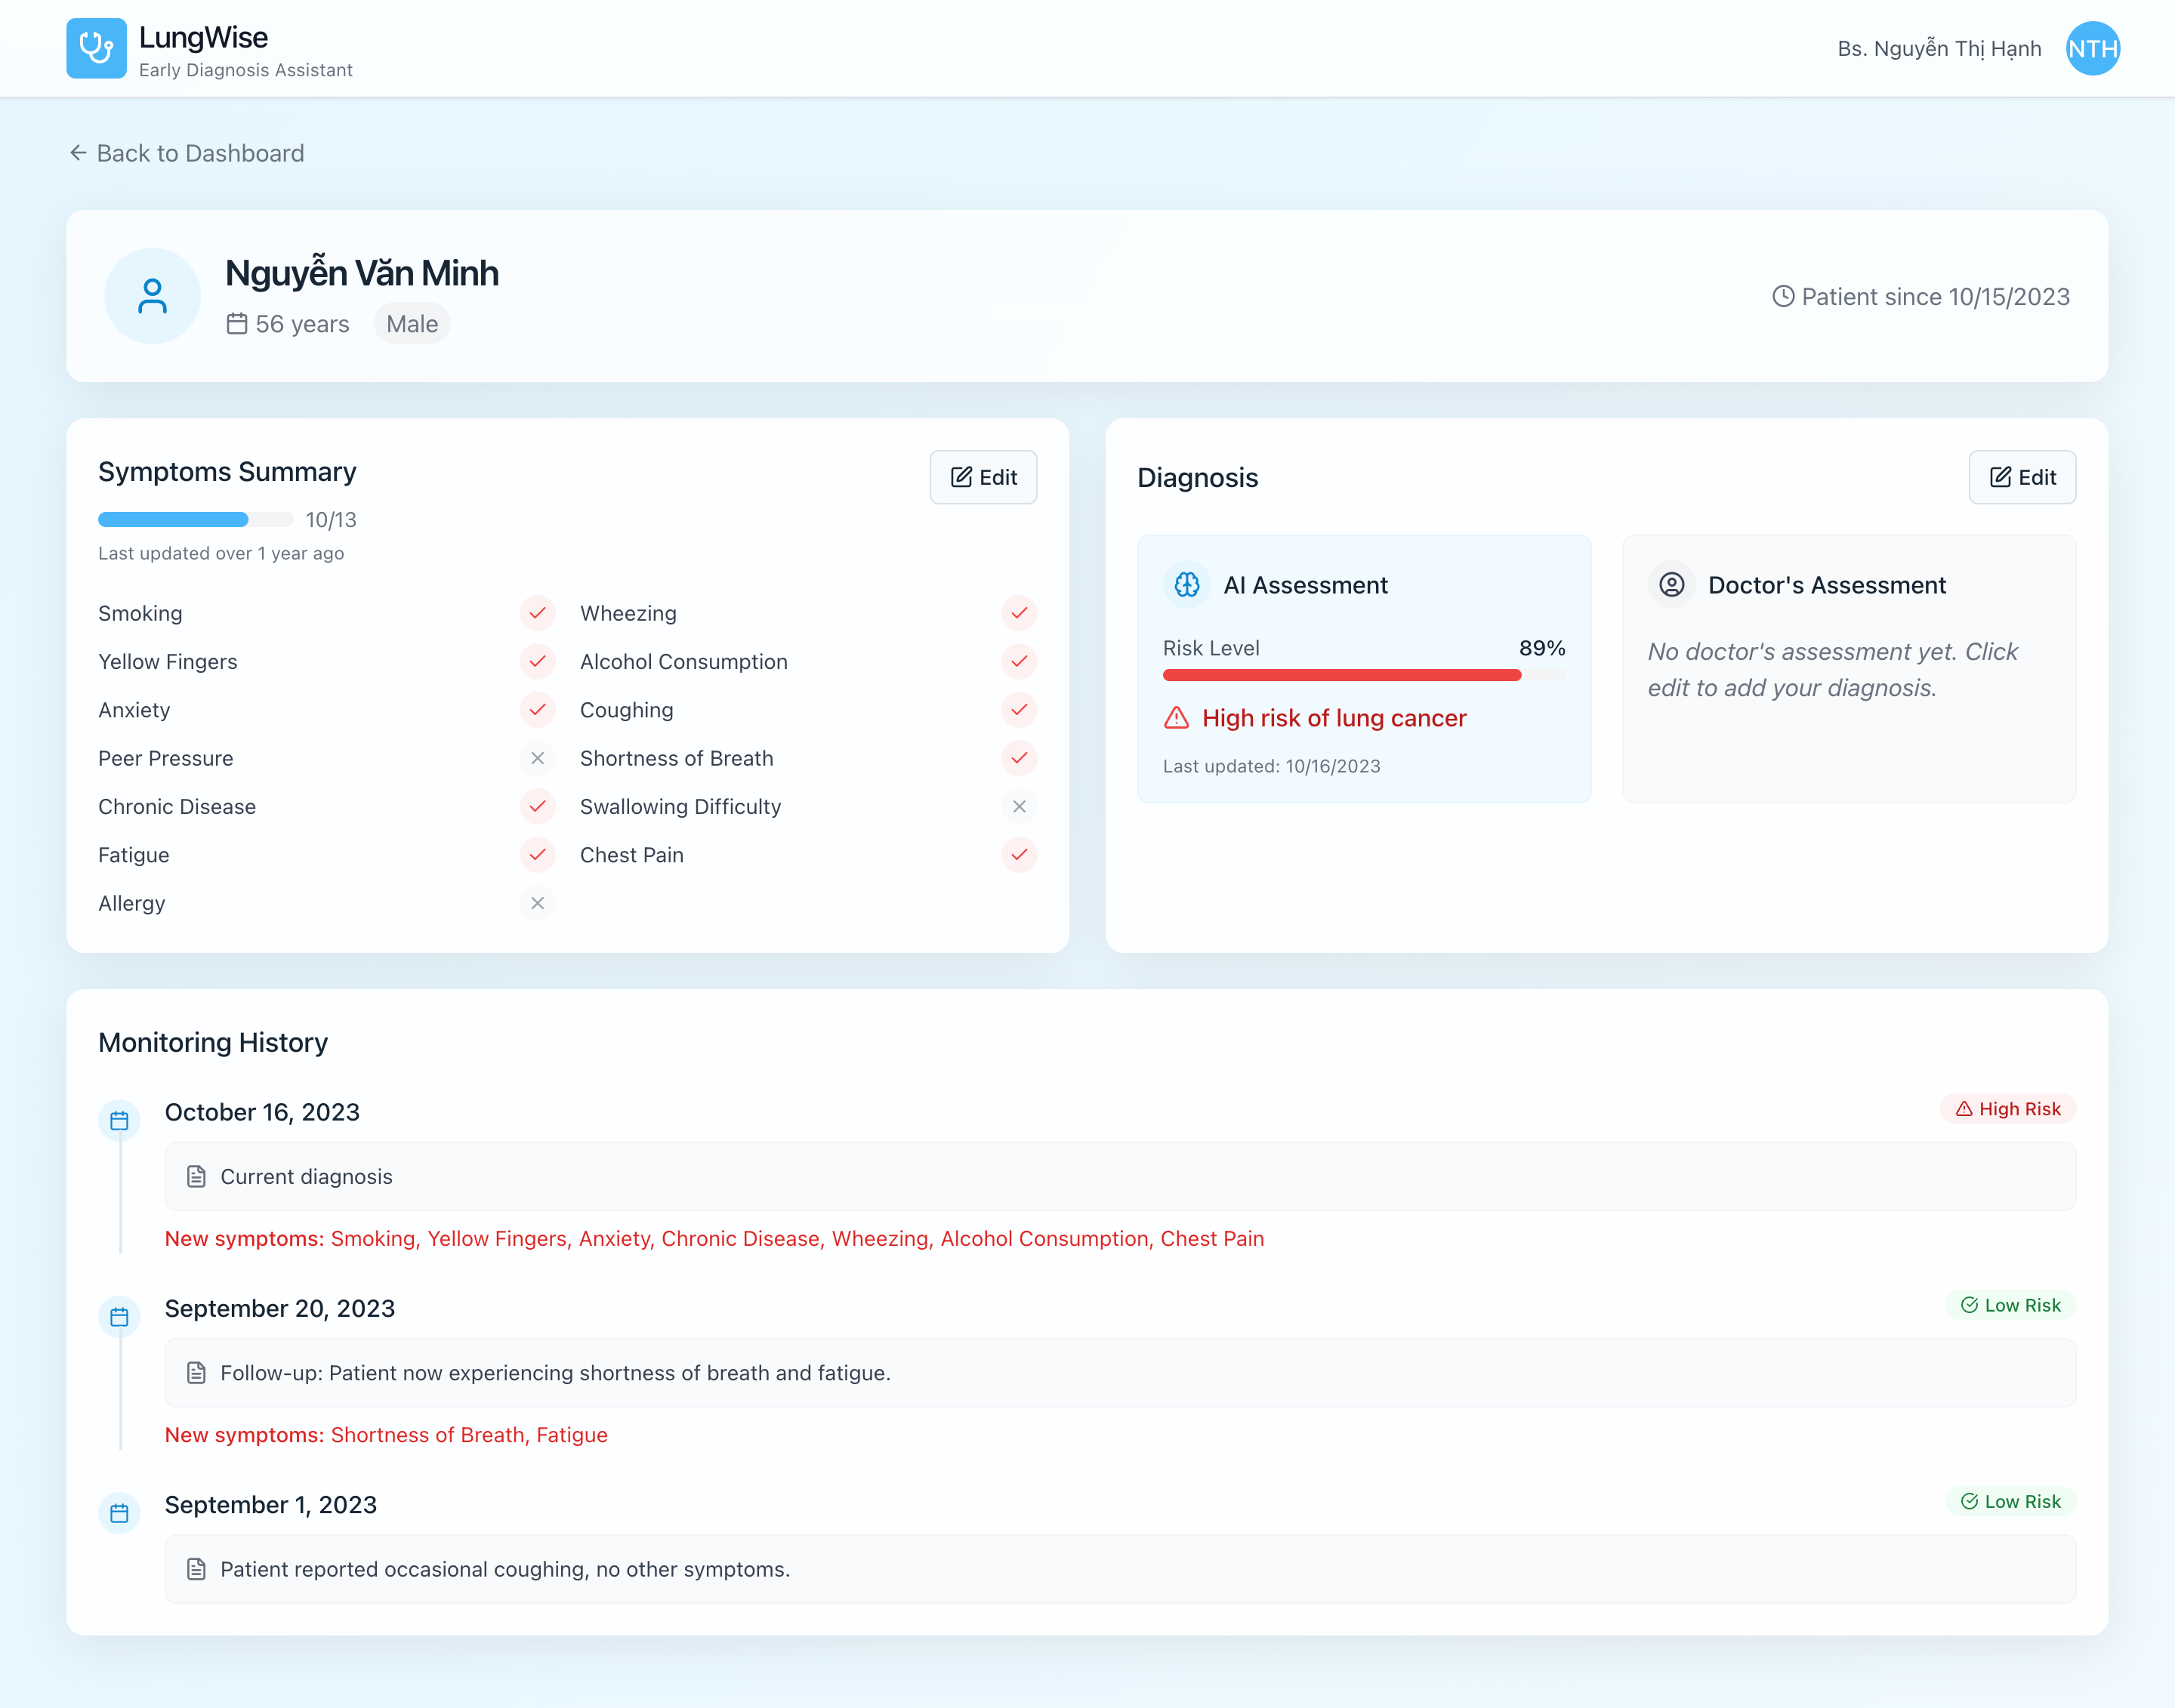
\includegraphics[width=0.9\textwidth]{Images/patient_detail.png}
    \caption{Patient detail interface showing personal information, symptoms summary, diagnostic assessment, and monitoring history.}
    \label{fig:patient_detail_mockup}
\end{figure}

\begin{figure}[h]
    \centering
    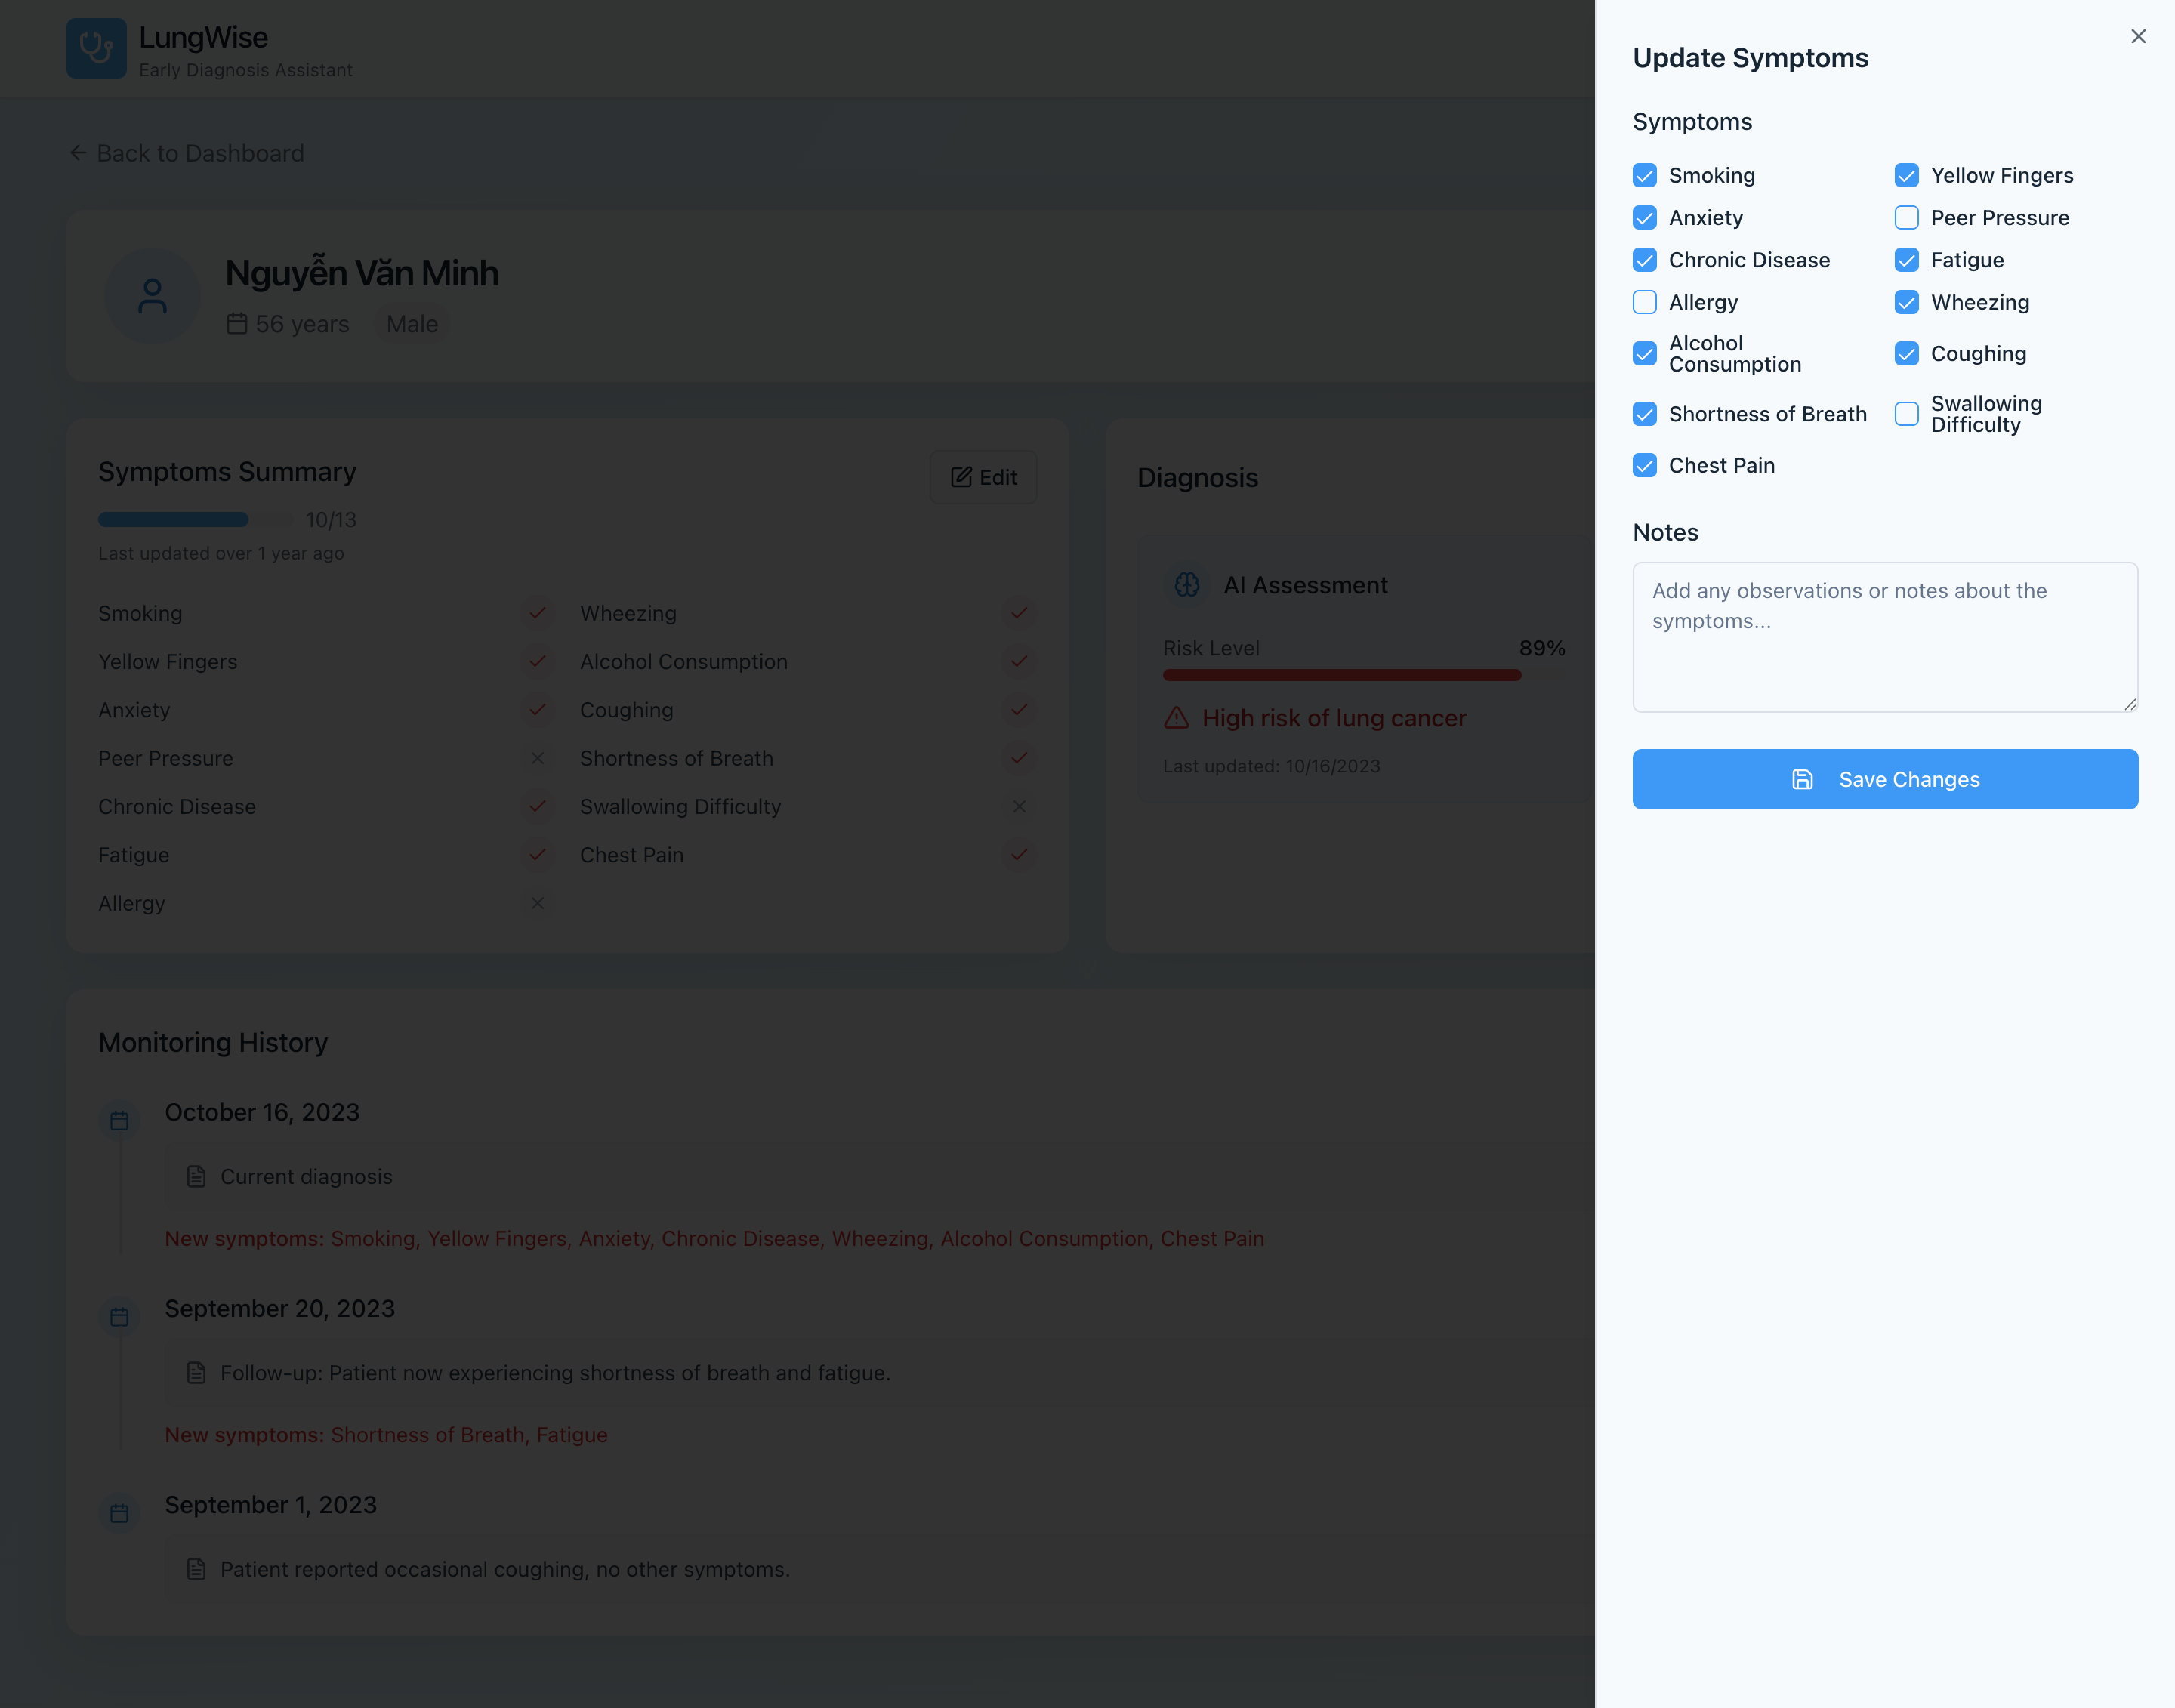
\includegraphics[width=0.9\textwidth]{Images/patient_update_symptoms.png}
    \caption{Patient symptom update interface allowing healthcare providers to record current symptoms and their severity.}
    \label{fig:symptom_update}
\end{figure}

\begin{figure}[h]
    \centering
    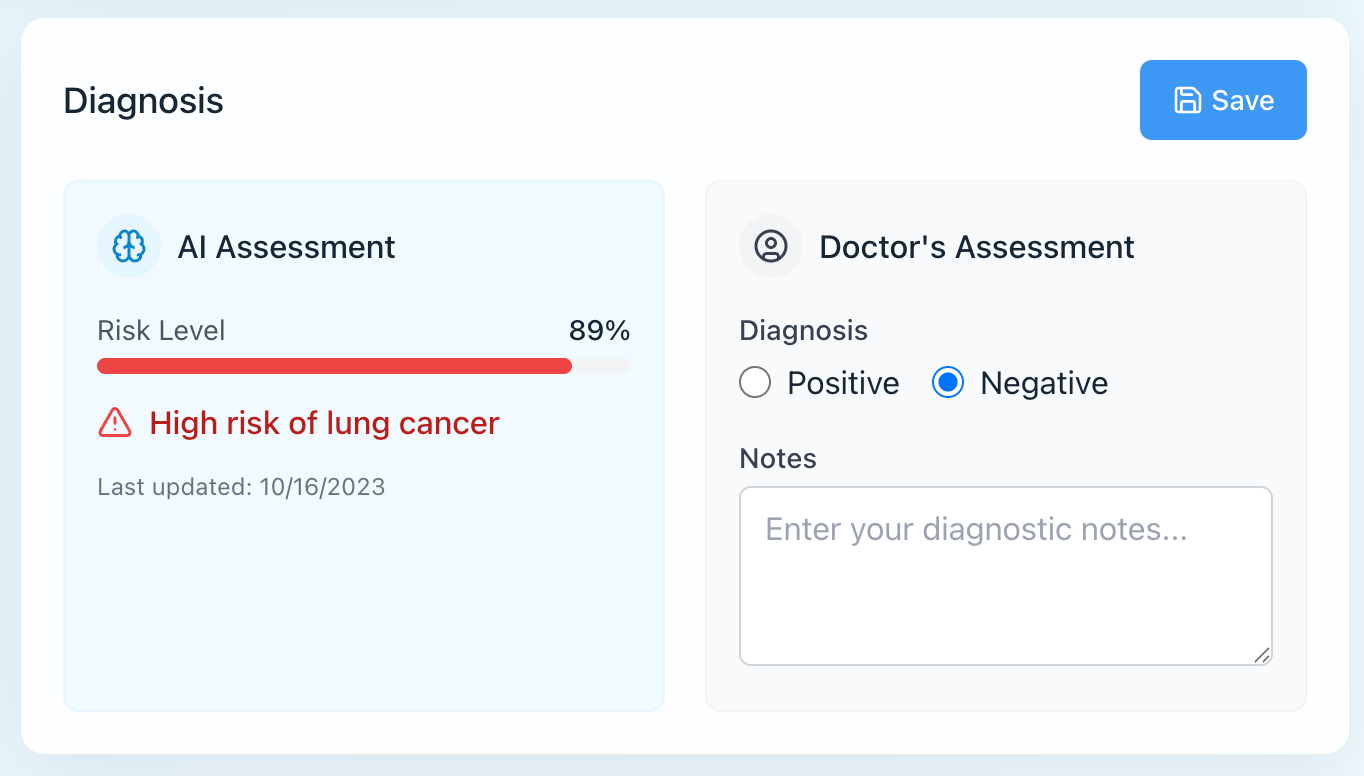
\includegraphics[width=0.9\textwidth]{Images/doctor_feedback_box.png}
    \caption{Doctor feedback interface where physicians can provide their clinical assessment and treatment recommendations based on updated symptoms and AI risk prediction.}
    \label{fig:doctor_feedback}
\end{figure}

\subsection{Backend Services}

The backend service plays a central role, handling business logic, data management, and interaction with the AI model. It provides a RESTful application programming interface (API) for the frontend to interact with.
\begin{itemize}
    \item \textbf{Core Technology:} FastAPI (Python). FastAPI was chosen for its high performance, modern syntax based on Python type hints, and ability to automatically generate API documentation (Swagger UI/ReDoc).
    \item \textbf{Deployment:} The backend system is packaged as Docker services, facilitating deployment, management, and scaling across different environments.
    \item \textbf{Key APIs:} The main RESTful endpoints include:
        \begin{itemize}
            \item \texttt{GET /patients}: Get a list of patients (supports search and filtering).
            \item \texttt{GET /patients/\{patient\_id\}}: Get detailed information about a specific patient.
            \item \texttt{POST /patients}: Create a new patient record.
            \item \texttt{PUT /patients/\{patient\_id\}}: Update patient information.
            \item \texttt{GET /patients/\{patient\_id\}/history}: Get monitoring history (diagnoses, old symptoms) of a patient.
            \item \texttt{POST /patients/\{patient\_id\}/diagnoses}: Add a new diagnosis record, including calling the AI model to get risk prediction and storing the results along with doctor's notes.
            \item \texttt{POST /patients/\{patient\_id\}/symptoms}: Update current patient symptoms.
            \item \texttt{POST /predict}: Receive patient data (features) and return lung cancer risk prediction from the XGBoost model. (Usually called internally when creating a new diagnosis, but can be provided separately if needed).
            \item \texttt{GET /model/info}: Get information about the ML model version being used (e.g., training date, key performance metrics).
            \item \texttt{POST /explain}: Receive patient data and return explanation for the prediction (e.g., using SHAP values to identify most influential features).
            \item \texttt{POST /retrain}: Trigger the ML model retraining process (typically protected and only for administrators or automated processes).
            \item \textit{(User authentication is handled through integrated Supabase Auth.)}
        \end{itemize}
    \end{itemize}
\end{itemize}

\subsection{Database}

The database stores all important information for the system.
\begin{itemize}
    \item \textbf{Database Management System:} PostgreSQL was chosen as the main relational database. PostgreSQL is known for its reliability, rich features, and scalability, making it suitable for storing structured data such as patient records, symptom logs, and monitoring events.
    \item \textbf{Real-time Updates:} Leveraging Supabase's real-time subscriptions feature (or a similar PostgreSQL-based solution) to push data updates (e.g., new prediction results, changed patient information) from backend to client automatically, ensuring the user interface always displays the latest information without manual refreshing.
\end{itemize}

\subsection{System Architecture Diagram}

Figure \ref{fig:system_architecture} illustrates the overall architecture and interaction between the different components of the LungWise application.

\begin{figure}[h]
    \centering
    \begin{tikzpicture}[
        node distance=1.5cm and 3cm,
        box/.style={draw, rounded corners, minimum width=3cm, minimum height=1.5cm, fill=blue!10, text width=3cm, align=center},
        arrow/.style={->, >=latex, thick},
        database/.style={cylinder, draw, shape border rotate=90, aspect=0.3, minimum width=1.5cm, minimum height=2cm, fill=green!10, text width=1.5cm, align=center},
        model/.style={ellipse, draw, minimum width=2cm, minimum height=1.5cm, fill=orange!20, text width=2.5cm, align=center}
    ]
    
    % Client tier
    \node[box, fill=blue!10] (ui) {User Interface\\(React, TypeScript)};
    \node[below=0.2cm of ui, align=center] (uitech) {\small Tailwind CSS\\Shadcn/UI};
    
    % Server tier
    \node[box, fill=purple!10, right=of ui] (api) {Backend API\\(FastAPI, Python)};
    \node[below=0.2cm of api, align=center] (apitech) {\small REST Endpoints\\JWT Auth};
    
    % Model tier
    \node[model, below right=of api] (model) {ML Model\\(XGBoost)};
    
    % Data tier
    \node[database, below left=of api] (db) {Database\\(PostgreSQL)};
    
    % Connections
    \draw[arrow] (ui) -- node[above] {\small HTTP/REST} (api);
    \draw[arrow] (api) -- node[left] {\small CRUD} (db);
    \draw[arrow] (db) -- node[below] {\small Patient Data} ([xshift=-1cm]api.south);
    \draw[arrow] (api) -- node[right] {\small Features} (model);
    \draw[arrow] (model) -- node[below] {\small Predictions} ([xshift=1cm]api.south);
    \draw[arrow] ([xshift=1.5cm]api.west) -- node[below] {\small JSON} ([xshift=-1.5cm]ui.east);
    
    % Real-time subscription
    \draw[arrow, dashed] (db) to[out=180, in=240] node[left] {\small Real-time\\Updates} (ui);
    
    % User
    \node[left=of ui, align=center] (user) {\includegraphics[width=1cm]{Images/doctor-icon.png}\\Doctor};
    \draw[arrow] (user) -- (ui);
    
    % System boundary
    \node[draw, dashed, fit=(ui) (uitech) (api) (apitech) (db) (model), inner sep=0.5cm, rounded corners] (system) {};
    \node[above] at (system.north) {LungWise System};
    
    \end{tikzpicture}
    \caption{System architecture diagram of the LungWise application showing the interaction between the user interface, backend services, machine learning model, and database.}
    \label{fig:system_architecture}
\end{figure}

As shown in the diagram, the LungWise system follows a modern three-tier architecture with clear separation of concerns:

\begin{itemize}
    \item The \textbf{Client Tier} consists of the React/TypeScript frontend that doctors interact with. It communicates with the backend via HTTP/REST calls and receives real-time updates through a subscription mechanism.
    
    \item The \textbf{Server Tier} contains the FastAPI backend that processes requests, enforces business logic, and orchestrates data flow between the client, database, and ML model.
    
    \item The \textbf{Data Tier} includes both the PostgreSQL database for persistent storage and the XGBoost model for risk predictions.
\end{itemize}

This architecture provides several advantages:
\begin{itemize}
    \item \textbf{Scalability:} Each component can be scaled independently based on demand.
    \item \textbf{Maintainability:} Changes to one tier (e.g., updating the ML model) can be made without affecting other tiers.
    \item \textbf{Security:} Sensitive operations and data access are handled on the server, not exposed to the client.
    \item \textbf{Real-time capabilities:} Users receive immediate updates when data changes.
\end{itemize}
